% =====================================================================
%  ESTUDO DE 26/10/2026: CAPÍTULO III COM JANELAS FIXAS (ARIMA 240, GARCH 500)
%  Não é texto do TG. Mesma estrutura do tg/conteudo/cap3-resultados.tex.
%
%  Procedência (E = dados/resultados/janelas_240_500_2026-10-26/; C = E/cru/,
%  gerado por ferramentas/scripts/estudo_janelas_dados.sh):
%   - Quadro das escolhas: E/escolhas/r3_C1..C3.txt e r6_C4.txt
%   - Tabelas de cada período: C/tabelas.txt (cru: ret, queda, vol, neg)
%   - Retorno por ano: C/anual_T1.csv, anual_T2.csv, anual_R6.csv, anual_T3.csv
%   - 2008 e 2020: C/recorte_2008.txt, C/recorte_2020.txt, C/curva_2008.csv,
%     C/curva_2020.csv, C/exposicao_2008.csv, C/exposicao_2020.csv,
%     C/exposicao_mensal_T1.txt, C/exposicao_mensal_2020.txt
%   - Saldo do MetaTrader 5: C/saldo_mt5.txt e E/relatorios_mt5/rel_*.png
%     (saldo final de cada relatório = 100000 × (1 + ret_puro), conferido)
%   - Efeito do GARCH (12 comparações): C/efeito_garch.txt
%   - Mecanismo (acerto, vetos, sinais, exposição): C/mecanismo.txt;
%     d = 1 e persistência do GARCH: C/traco_resumo.txt; 03/04/2020: traço
%     (C/traco_resumo.txt) e dados/series/PETR4_OFICIAL.csv (15,51 / 30,18)
%   - Quatro ações (dois grupos) e venda a descoberto:
%     C/analise_grades_cru.txt, blocos 2, 3 e 6
%   - Outras ações: C/outras_acoes.txt
%   - Comparação com o TG: E/comparacao_tg.txt e C/efeito_janela_garch.txt
%   - Queda da PETR4 em 2018: C/petr4_2018.txt
% =====================================================================
\setdiv{CAPÍTULO III}
\chapter{Análise e discussão dos dados com janelas fixas}

Este capítulo repete o Capítulo III com o ARIMA estimado sempre sobre 240
pregões e o GARCH sobre 500 resíduos. A ordem é a mesma. Começa pela reprodução
do estudo de \citeonline{almeida2016}, apresenta cada período de teste com o ano
de cada crise em detalhe, verifica se o efeito vem do GARCH, mostra como ele
protege o capital e fecha com as outras três ações. A última seção compara estes
resultados com os da versão atual.

\section{Reprodução do estudo de referência}

A reprodução do estudo de \citeonline{almeida2016} usa apenas as médias móveis,
que não dependem das janelas do ARIMA e do GARCH. Ela é, portanto, a mesma do
Capítulo III, e as médias móveis reproduzidas das seções seguintes também são as
mesmas.

\section{Como os resultados são apresentados}

A apresentação segue a do Capítulo III. Cada período tem uma tabela com o
resultado bruto de cada robô, um gráfico com a evolução do patrimônio e o saldo
registrado pelo MetaTrader 5 para o ARIMA e para o ARIMA-GARCH. Nos períodos com
crise, o ano da crise é apresentado em seguida, como recorte do mesmo teste.

A escolha das configurações foi refeita com a nova grade, e o resultado mudou. O
Quadro~\ref{qua:escolhas-j} mostra o que cada versão faz em cada período. Em
sete dos dez casos o veto mantém a posição aberta, e em dois o limiar é um
valor fixo de 2\% ao dia, em vez do percentil da volatilidade.

% Procedência: E/escolhas/r3_C1..C3.txt (2007-2011, 2013-2016, 2025-2026, e
% fixas = C2) e r6_C4.txt (2017-2024). Estrategia 0 = filtro, 3 = filtro e
% ajuste; ModoLimiar 0 = absoluto (Limiar_Absoluto 0,02), 1 = percentil.
\begin{quadro}[htbp]
\centering
\caption{Forma de uso do GARCH em cada robô escolhido, com janelas fixas}
\label{qua:escolhas-j}
\fontsize{10}{12}\selectfont
\begin{tabular}{|>{\raggedright\arraybackslash}p{3.4cm}|>{\raggedright\arraybackslash}p{5.4cm}|>{\raggedright\arraybackslash}p{5.4cm}|}
\hline
Período de teste & ARIMA-GARCH Sharpe & ARIMA-GARCH Calmar \\
\hline
2007 a 2011 & filtro e ajuste da posição, mantém a posição no veto & filtro e ajuste da posição, encerra a posição no veto \\
\hline
2013 a 2016 & filtro, mantém a posição no veto & filtro e ajuste da posição, mantém a posição no veto \\
\hline
2017 a 2024 & filtro, encerra a posição no veto & filtro e ajuste da posição com limiar fixo, encerra a posição no veto \\
\hline
2025 a 2026 & filtro, mantém a posição no veto & filtro e ajuste da posição com limiar fixo, mantém a posição no veto \\
\hline
2005 a 2026 e 2017 a 2024, fixas & filtro, mantém a posição no veto & filtro e ajuste da posição, mantém a posição no veto \\
\hline
\end{tabular}
\fonte{Elaboração própria.}
\end{quadro}

\section{Crise financeira, 2007 a 2011}

\subsection{O período completo}

A Tabela~\ref{tab:crise-j} apresenta o resultado do primeiro período. Desta vez,
os dois critérios escolheram configurações diferentes, que diferem apenas no veto.
O ARIMA-GARCH Sharpe mantém a posição aberta, e o ARIMA-GARCH Calmar a encerra.

\begin{table}[htbp]
\centering
\caption{Resultado de 2007 a 2011, com janelas fixas}
\label{tab:crise-j}
\fontsize{10}{12}\selectfont
\begin{tabular}{l|c|c|c|c}
\hline
Robô & Retorno & Queda máx. & Volatilidade & Negociações \\
\hline
Médias móveis reproduzidas & $-$31,6\% & 64,6\% & 28,7\% & 31 \\
\hline
ARIMA & $-$12,7\% & 45,1\% & 27,5\% & 320 \\
\hline
ARIMA-GARCH Sharpe & +31,4\% & 13,5\% & 12,7\% & 208 \\
\hline
ARIMA-GARCH Calmar & +1,7\% & 10,1\% & 8,4\% & 215 \\
\hline
PETR4 & $-$14,0\% & 67,2\% & 43,2\% & -- \\
\hline
\end{tabular}
\fonte{Elaboração própria.}
\nota{Resultado bruto. Neste período, o ARIMA é a mesma configuração das duas versões com o GARCH desligado.}
\end{table}

As duas versões com GARCH foram as únicas com ganho e as que menos caíram. O
ARIMA-GARCH Sharpe ganhou 31,4\% com queda máxima de 13,5\%, enquanto a PETR4
perdeu 14,0\% e chegou a cair 67,2\%. O ARIMA-GARCH Calmar praticamente empatou,
com ganho de 1,7\%, mas teve a menor queda e a menor volatilidade do período.
Como o ARIMA é, aqui, a mesma configuração com o GARCH desligado, a diferença
entre ele e as duas versões vem apenas do GARCH.

O Gráfico~\ref{gra:anual-t1-j} mostra que a vantagem do ARIMA-GARCH Sharpe veio
principalmente de 2007, quando ganhou 20,9\%, e de 2008, quando perdeu apenas
1,7\%. A proteção custou nos anos de alta. Em 2009, a ação subiu 61,1\% e o
ARIMA, 33,6\%, enquanto as duas versões com GARCH ganharam cerca de 8\%.

\begin{grafico}[htbp]
\centering
\caption{Retorno por ano, 2007 a 2011, com janelas fixas}
\label{gra:anual-t1-j}
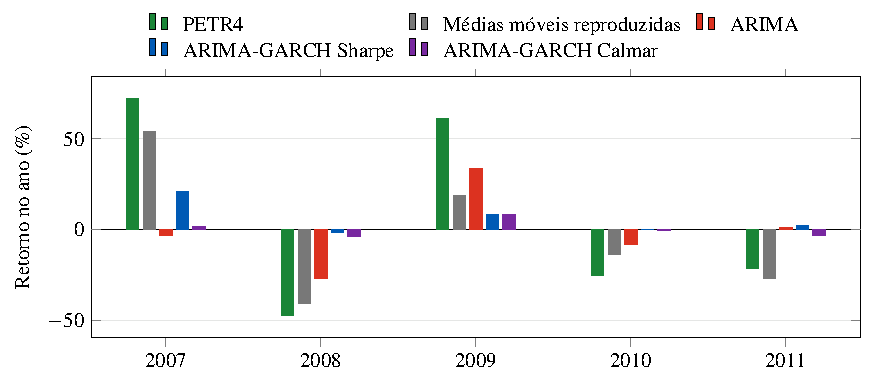
\includegraphics{anual_T1.pdf}
\fonte{Elaboração própria.}
\nota{Resultado bruto.}
\end{grafico}

O Gráfico~\ref{gra:curva-t1-j} mostra a evolução do patrimônio e a queda
acumulada de cada robô ao longo dos cinco anos.

\begin{grafico}[htbp]
\centering
\caption{Patrimônio e queda acumulada, 2007 a 2011, com janelas fixas}
\label{gra:curva-t1-j}
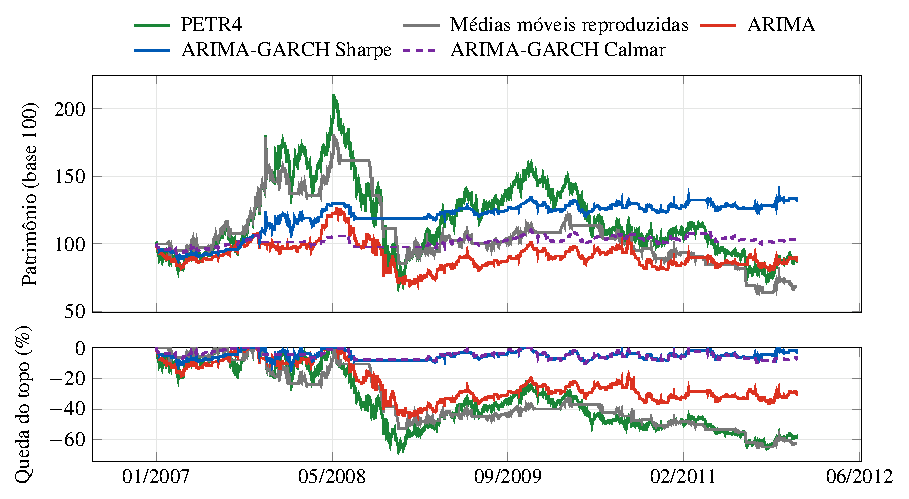
\includegraphics{curva_T1.pdf}
\fonte{Elaboração própria.}
\nota{Resultado bruto, com o capital inicial igual a 100.}
\end{grafico}

No saldo registrado pelo MetaTrader 5, no Gráfico~\ref{gra:mt5-t1-j}, o ARIMA
subiu até R\$ 126 mil em maio de 2008 e desceu a R\$ 71 mil em dezembro do mesmo
ano. O saldo do ARIMA-GARCH Sharpe ficou entre R\$ 89 mil, logo no início do
teste, e R\$ 134 mil, em dezembro de 2009.

\begin{grafico}[htbp]
\centering
\caption{Saldo registrado pelo MetaTrader 5, 2007 a 2011, com janelas fixas}
\label{gra:mt5-t1-j}
{\small ARIMA}\\[2pt]
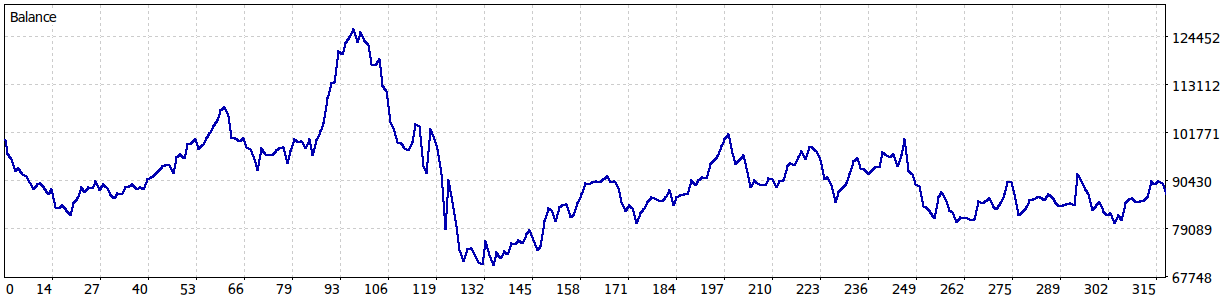
\includegraphics[width=0.7\textwidth]{../relatorios_mt5/rel_R3_T1_AS.png}\\[6pt]
{\small ARIMA-GARCH Sharpe}\\[2pt]
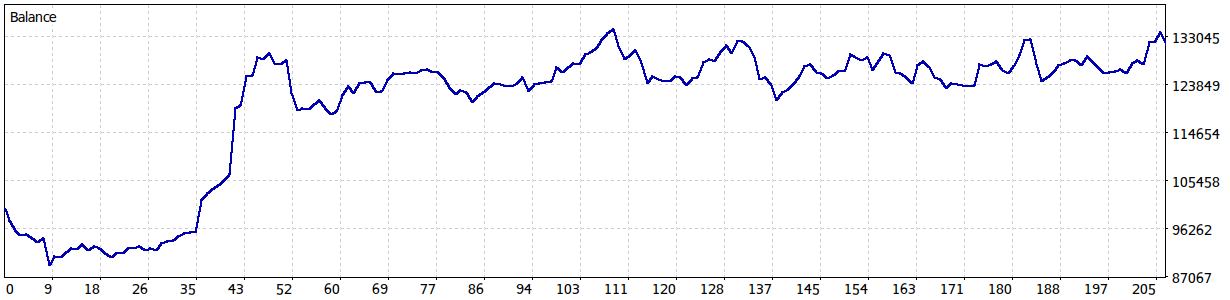
\includegraphics[width=0.7\textwidth]{../relatorios_mt5/rel_R3_T1_GS.png}
\fonte{Relatório do testador de estratégias do MetaTrader 5.}
\nota{Saldo em reais após cada negociação encerrada. O eixo horizontal é o número da negociação, e as escalas dos dois painéis são diferentes.}
\end{grafico}

\FloatBarrier
\subsection{O ano de 2008}

Os números da Tabela~\ref{tab:ano-2008-j} são um recorte do teste de 2007 a 2011,
com as configurações escolhidas em 2005 e 2006, antes da crise.

\begin{table}[htbp]
\centering
\caption{Resultado em 2008, ano da crise financeira, com janelas fixas}
\label{tab:ano-2008-j}
\fontsize{10}{12}\selectfont
\begin{tabular}{l|c|c}
\hline
Robô & Retorno no ano & Queda máx. no ano \\
\hline
Médias móveis reproduzidas & $-$40,7\% & 52,5\% \\
\hline
ARIMA & $-$27,1\% & 45,2\% \\
\hline
ARIMA-GARCH Sharpe & $-$1,7\% & 11,9\% \\
\hline
ARIMA-GARCH Calmar & $-$3,6\% & 7,6\% \\
\hline
PETR4 & $-$47,3\% & 67,2\% \\
\hline
\end{tabular}
\fonte{Elaboração própria.}
\nota{Resultado bruto. A queda máxima é medida dentro do ano, a partir do fechamento de 2007.}
\end{table}

Enquanto a PETR4 perdia 47,3\%, as duas versões com GARCH terminaram o ano
perto do zero, com perdas de 1,7\% e 3,6\%, contra 27,1\% do ARIMA e 40,7\% das
médias móveis. A maior queda dentro do ano foi de 11,9\% no ARIMA-GARCH Sharpe e
de 7,6\% no ARIMA-GARCH Calmar, contra 45,2\% do ARIMA, que é a mesma configuração
sem o GARCH.

\begin{grafico}[htbp]
\centering
\caption{Patrimônio e queda acumulada, 2008, com janelas fixas}
\label{gra:curva-2008-j}
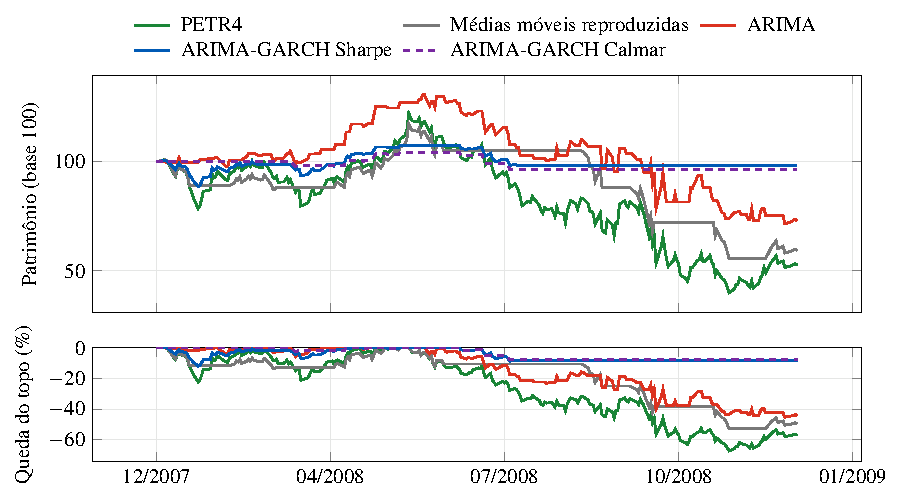
\includegraphics{curva_2008.pdf}
\fonte{Elaboração própria.}
\nota{Resultado bruto, com o patrimônio no fim de 2007 igual a 100. A queda é medida dentro do ano.}
\end{grafico}

O Gráfico~\ref{gra:curva-2008-j} mostra a evolução do patrimônio ao longo do ano,
e o Gráfico~\ref{gra:exposicao-2008-j}, quanto dele cada robô manteve aplicado.
O ARIMA-GARCH Sharpe começou o ano com mais da metade do patrimônio aplicado,
51,2\% em média em janeiro, mais que o ARIMA. A partir de março, a sua posição
foi reduzida, e de agosto a dezembro ele ficou inteiramente fora do mercado. Em
outubro, mês em que a ação caiu 32,8\%, o ARIMA manteve, em média, 56,4\% do
patrimônio aplicado.

\begin{grafico}[htbp]
\centering
\caption{Preço da PETR4 e patrimônio aplicado na ação, 2008, com janelas fixas}
\label{gra:exposicao-2008-j}
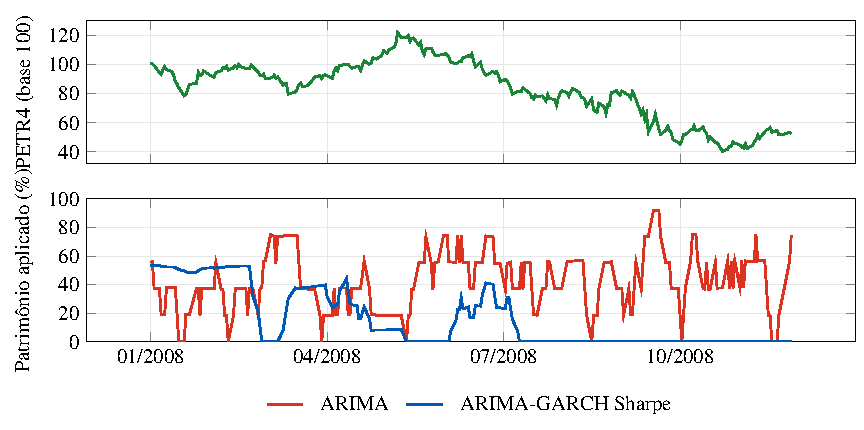
\includegraphics{exposicao_2008.pdf}
\fonte{Elaboração própria.}
\nota{O patrimônio aplicado é a média dos cinco pregões anteriores, cerca de uma semana. O ARIMA é a mesma configuração do ARIMA-GARCH Sharpe com o GARCH desligado. O preço da PETR4 tem base 100 no fim de 2007.}
\end{grafico}

\section{Queda prolongada e recuperação, 2013 a 2016}

A Tabela~\ref{tab:fora-crise-j} apresenta o resultado do segundo período.

\begin{table}[htbp]
\centering
\caption{Resultado de 2013 a 2016, com janelas fixas}
\label{tab:fora-crise-j}
\fontsize{10}{12}\selectfont
\begin{tabular}{l|c|c|c|c}
\hline
Robô & Retorno & Queda máx. & Volatilidade & Negociações \\
\hline
Médias móveis reproduzidas & +100,8\% & 42,0\% & 40,4\% & 24 \\
\hline
ARIMA & $-$50,4\% & 63,8\% & 38,2\% & 127 \\
\hline
ARIMA-GARCH Sharpe & $-$24,5\% & 77,6\% & 47,2\% & 141 \\
\hline
ARIMA-GARCH Calmar & $-$9,6\% & 40,5\% & 16,6\% & 141 \\
\hline
PETR4 & $-$25,6\% & 83,1\% & 59,2\% & -- \\
\hline
\end{tabular}
\fonte{Elaboração própria.}
\nota{Resultado bruto.}
\end{table}

As médias móveis tiveram de novo o melhor resultado, com ganho de 100,8\%. O
ARIMA-GARCH Calmar perdeu pouco e foi o que menos caiu e menos oscilou. O
ARIMA-GARCH Sharpe, ao contrário, teve a maior queda máxima entre os robôs,
77,6\%, e a maior volatilidade. Ele usa só o filtro e mantém a posição aberta
durante o veto. Nos dias de volatilidade alta, deixa de agir, inclusive para
vender, e por isso ficou, em média, com 59,4\% do patrimônio aplicado, mais que a
mesma configuração sem o GARCH, com 49,5\%.

O Gráfico~\ref{gra:anual-t2-j} mostra que as médias móveis perderam dinheiro de
2013 a 2015 e ganharam 194,5\% em 2016, quando a ação subiu 123,3\%. O
ARIMA-GARCH Sharpe perdeu 36,8\% em 2014 e 24,4\% em 2015 e recuperou parte em
2016, com ganho de 73,3\%.

\begin{grafico}[htbp]
\centering
\caption{Retorno por ano, 2013 a 2016, com janelas fixas}
\label{gra:anual-t2-j}
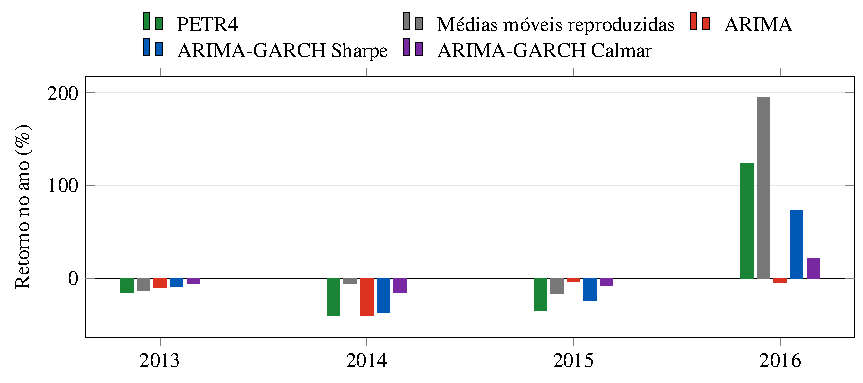
\includegraphics{anual_T2.pdf}
\fonte{Elaboração própria.}
\nota{Resultado bruto.}
\end{grafico}

\begin{grafico}[htbp]
\centering
\caption{Patrimônio e queda acumulada, 2013 a 2016, com janelas fixas}
\label{gra:curva-t2-j}
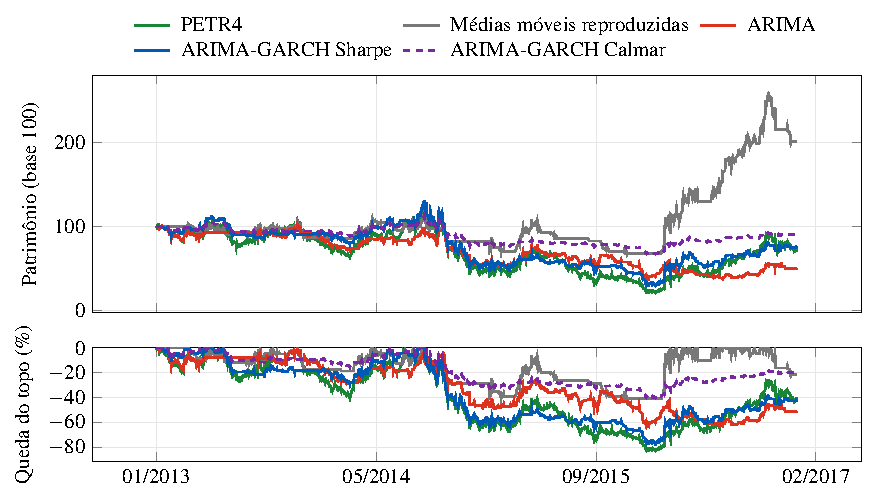
\includegraphics{curva_T2.pdf}
\fonte{Elaboração própria.}
\nota{Resultado bruto, com o capital inicial igual a 100.}
\end{grafico}

O Gráfico~\ref{gra:curva-t2-j} mostra a evolução do patrimônio. No saldo
registrado pelo MetaTrader 5, no Gráfico~\ref{gra:mt5-t2-j}, o ARIMA chegou a
R\$ 38 mil em julho de 2016, e o ARIMA-GARCH Sharpe, a R\$ 43 mil em janeiro do
mesmo ano.

\begin{grafico}[htbp]
\centering
\caption{Saldo registrado pelo MetaTrader 5, 2013 a 2016, com janelas fixas}
\label{gra:mt5-t2-j}
{\small ARIMA}\\[2pt]
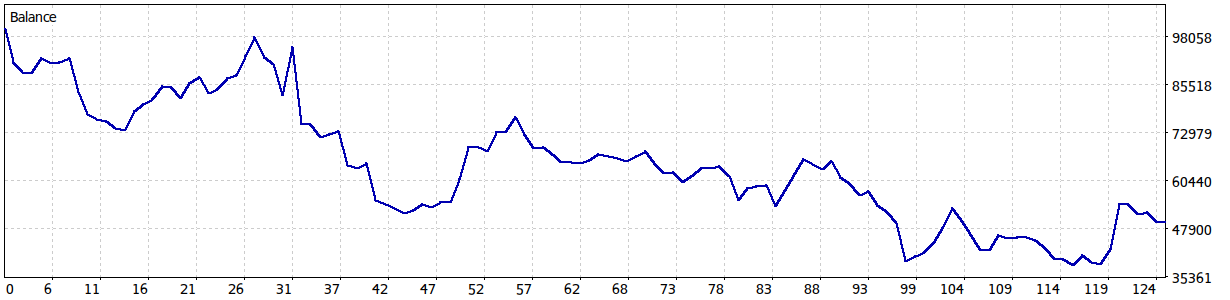
\includegraphics[width=0.7\textwidth]{../relatorios_mt5/rel_R3_T2_AS.png}\\[6pt]
{\small ARIMA-GARCH Sharpe}\\[2pt]
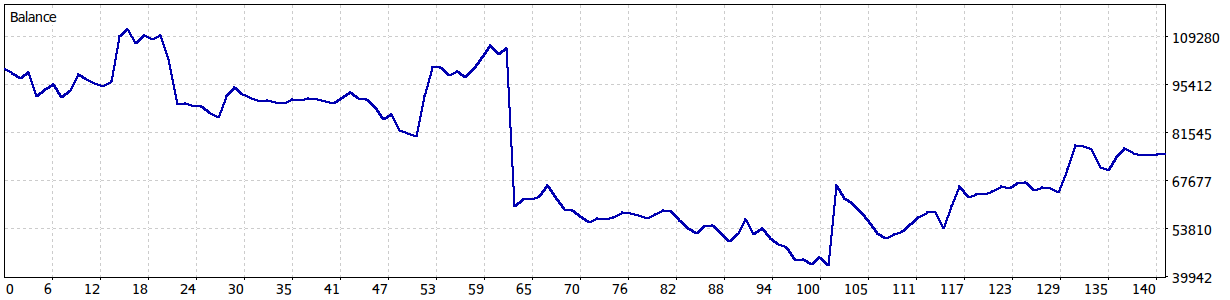
\includegraphics[width=0.7\textwidth]{../relatorios_mt5/rel_R3_T2_GS.png}
\fonte{Relatório do testador de estratégias do MetaTrader 5.}
\nota{Saldo em reais após cada negociação encerrada. O eixo horizontal é o número da negociação, e as escalas dos dois painéis são diferentes.}
\end{grafico}

\section{Teste principal, 2017 a 2024}

\subsection{O período completo}

A Tabela~\ref{tab:principal-j} apresenta o resultado do teste principal.

\begin{table}[htbp]
\centering
\caption{Resultado de 2017 a 2024, com janelas fixas}
\label{tab:principal-j}
\fontsize{10}{12}\selectfont
\begin{tabular}{l|c|c|c|c}
\hline
Robô & Retorno & Queda máx. & Volatilidade & Negociações \\
\hline
Médias móveis reproduzidas & +47,8\% & 37,9\% & 30,9\% & 56 \\
\hline
ARIMA & +95,7\% & 40,5\% & 32,0\% & 244 \\
\hline
ARIMA-GARCH Sharpe & +64,6\% & 37,0\% & 26,9\% & 247 \\
\hline
ARIMA-GARCH Calmar & $-$15,4\% & 21,6\% & 4,4\% & 111 \\
\hline
PETR4 & +143,6\% & 64,2\% & 44,8\% & -- \\
\hline
\end{tabular}
\fonte{Elaboração própria.}
\nota{Resultado bruto. O ARIMA é a mesma configuração do ARIMA-GARCH Sharpe com o GARCH desligado.}
\end{table}

Nenhum robô rendeu mais que a ação, que subiu 143,6\%. O ARIMA teve o maior
retorno entre eles, 95,7\%. O ARIMA-GARCH Sharpe, que é o mesmo ARIMA com o filtro,
rendeu 64,6\% e caiu um pouco menos, 37,0\% contra 40,5\%. O ARIMA-GARCH Calmar
quase não operou. Ele usa um limiar fixo de 2\% ao dia, vetou 1.597 dos 1.977
sinais do ARIMA e manteve, em média, só 4,4\% do patrimônio aplicado. Por isso
oscilou muito pouco, mas terminou o período com perda de 15,4\%.

\begin{grafico}[htbp]
\centering
\caption{Patrimônio e queda acumulada, 2017 a 2024, com janelas fixas}
\label{gra:curva-r6-j}
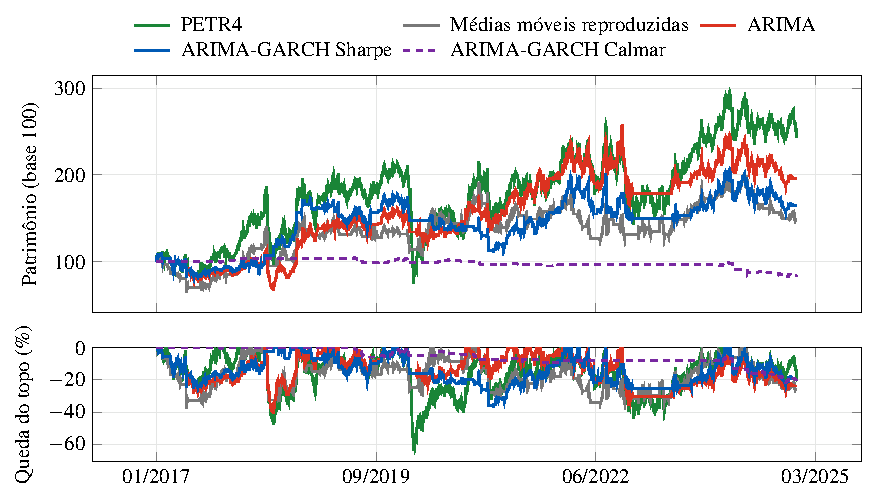
\includegraphics{curva_R6.pdf}
\fonte{Elaboração própria.}
\nota{Resultado bruto, com o capital inicial igual a 100.}
\end{grafico}

O Gráfico~\ref{gra:curva-r6-j} mostra a evolução do patrimônio, e o
Gráfico~\ref{gra:anual-r6-j}, o resultado de cada ano. O ARIMA-GARCH Sharpe foi o
robô que mais ganhou em 2018, 76,7\%, contra 50,1\% do ARIMA, e o que mais perdeu
em 2020, 21,4\%. Nos demais anos, ficou abaixo do ARIMA em 2019 e 2021 e próximo
dele nos outros.

\begin{grafico}[htbp]
\centering
\caption{Retorno por ano, 2017 a 2024, com janelas fixas}
\label{gra:anual-r6-j}
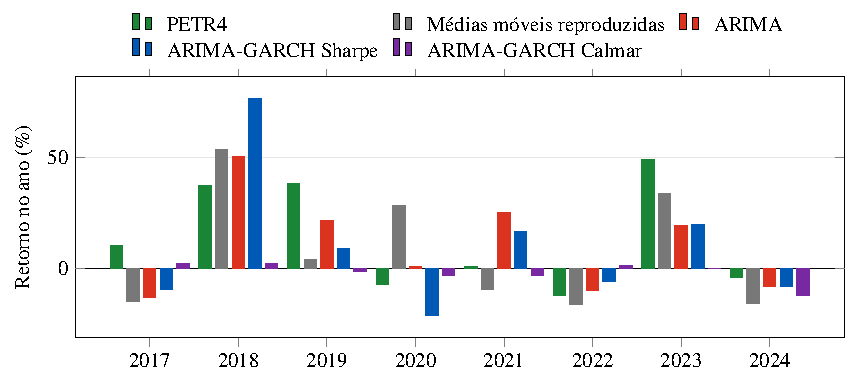
\includegraphics{anual_R6.pdf}
\fonte{Elaboração própria.}
\nota{Resultado bruto.}
\end{grafico}

No saldo registrado pelo MetaTrader 5, no Gráfico~\ref{gra:mt5-r6-j}, a queda mais
forte do ARIMA aconteceu em junho de 2018, quando a PETR4 perdeu 47,9\% do valor
em cerca de um mês, e levou o seu saldo a R\$ 69 mil. O menor saldo do ARIMA-GARCH
Sharpe, de R\$ 83 mil, foi registrado em julho de 2017, no início do teste. Ao fim
do período, o seu saldo era de R\$ 165 mil, contra R\$ 196 mil do ARIMA.

\begin{grafico}[htbp]
\centering
\caption{Saldo registrado pelo MetaTrader 5, 2017 a 2024, com janelas fixas}
\label{gra:mt5-r6-j}
{\small ARIMA}\\[2pt]
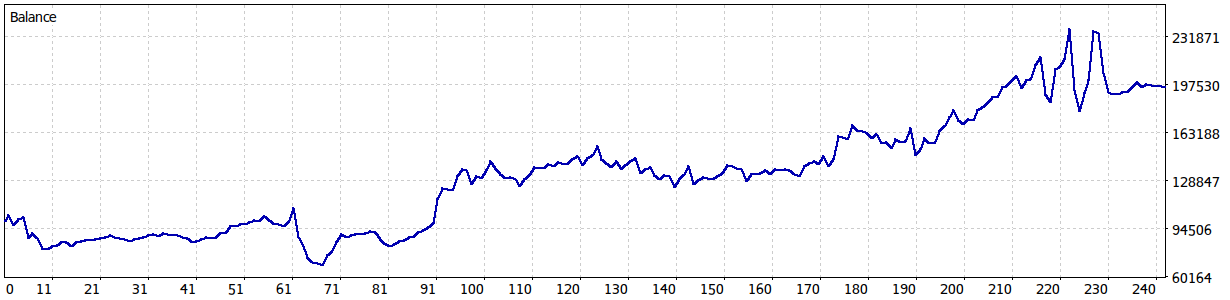
\includegraphics[width=0.7\textwidth]{../relatorios_mt5/rel_R6_ARIMA.png}\\[6pt]
{\small ARIMA-GARCH Sharpe}\\[2pt]
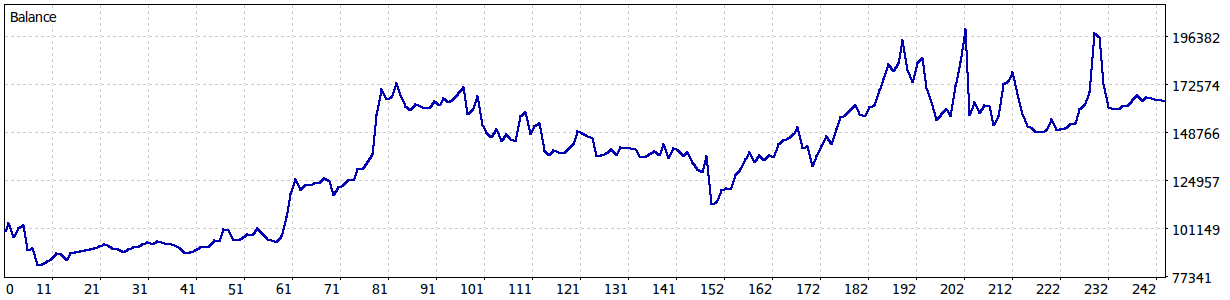
\includegraphics[width=0.7\textwidth]{../relatorios_mt5/rel_R6_GS.png}
\fonte{Relatório do testador de estratégias do MetaTrader 5.}
\nota{Saldo em reais após cada negociação encerrada. O eixo horizontal é o número da negociação, e as escalas dos dois painéis são diferentes.}
\end{grafico}

\FloatBarrier
\subsection{O ano de 2020}

Os números da Tabela~\ref{tab:pandemia-j} são um recorte do teste de 2017 a 2024,
com as configurações escolhidas em 2014 a 2016, antes da pandemia.

\begin{table}[htbp]
\centering
\caption{Resultado em 2020, ano da pandemia, com janelas fixas}
\label{tab:pandemia-j}
\fontsize{10}{12}\selectfont
\begin{tabular}{l|c|c}
\hline
Robô & Retorno no ano & Queda máx. no ano \\
\hline
Médias móveis reproduzidas & +28,2\% & 19,1\% \\
\hline
ARIMA & +0,7\% & 23,3\% \\
\hline
ARIMA-GARCH Sharpe & $-$21,4\% & 22,7\% \\
\hline
ARIMA-GARCH Calmar & $-$3,5\% & 4,7\% \\
\hline
PETR4 & $-$7,2\% & 64,2\% \\
\hline
\end{tabular}
\fonte{Elaboração própria.}
\nota{Resultado bruto. A queda máxima é medida dentro do ano, a partir do fechamento de 2019.}
\end{table}

A PETR4 chegou a perder 64,2\% do seu valor e terminou 2020 com queda de 7,2\%.
As médias móveis tiveram o melhor resultado, com ganho de 28,2\%. O ARIMA-GARCH
Sharpe teve queda máxima parecida com a do ARIMA, 22,7\% contra 23,3\%, mas
terminou o ano com perda de 21,4\%, enquanto o ARIMA ficou no zero. O ARIMA-GARCH
Calmar, quase sempre fora do mercado, perdeu 3,5\%. A mesma configuração do
ARIMA-GARCH Calmar sem o GARCH perdeu 36,9\% no ano e chegou a cair 55,3\%.

\begin{grafico}[htbp]
\centering
\caption{Patrimônio e queda acumulada, 2020, com janelas fixas}
\label{gra:curva-2020-j}
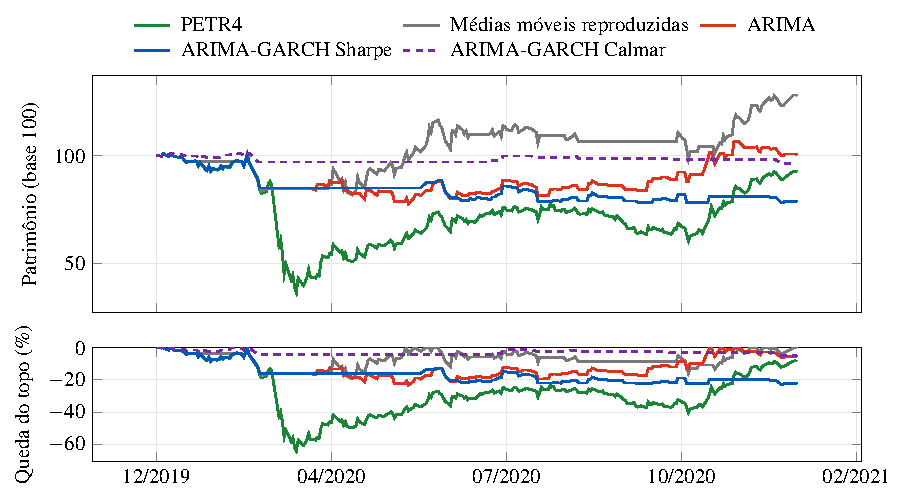
\includegraphics{curva_2020.pdf}
\fonte{Elaboração própria.}
\nota{Resultado bruto, com o patrimônio no fim de 2019 igual a 100. A queda é medida dentro do ano.}
\end{grafico}

O Gráfico~\ref{gra:curva-2020-j} mostra a evolução do patrimônio, e o
Gráfico~\ref{gra:exposicao-2020-j}, quanto dele cada robô manteve aplicado. Em
janeiro e fevereiro, o ARIMA e o ARIMA-GARCH Sharpe tinham quase todo o
patrimônio aplicado e perderam o mesmo, 6,0\% e 9,6\%. Em março, mês em que a
ação caiu 45,9\%, os dois ficaram praticamente fora. A diferença veio depois. Em
abril e maio, o GARCH manteve o robô inteiramente fora, enquanto o ARIMA voltou a
comprar. Em novembro, mês em que a ação subiu 32,0\%, o ARIMA ganhou 13,7\%, e o
ARIMA-GARCH Sharpe, com 4,7\% do patrimônio aplicado em média, ganhou 3,4\%. As
perdas do ARIMA-GARCH Sharpe no ano vieram de janeiro e fevereiro, antes da queda,
e de junho e agosto.

\begin{grafico}[htbp]
\centering
\caption{Preço da PETR4 e patrimônio aplicado na ação, 2020, com janelas fixas}
\label{gra:exposicao-2020-j}
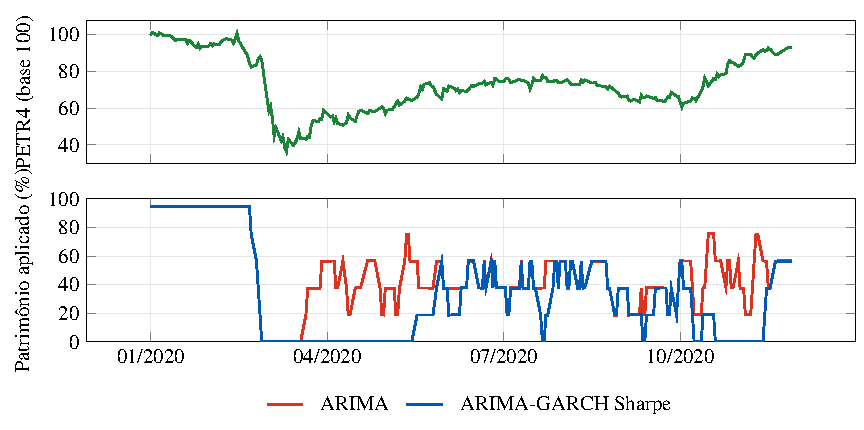
\includegraphics{exposicao_2020.pdf}
\fonte{Elaboração própria.}
\nota{O patrimônio aplicado é a média dos cinco pregões anteriores, cerca de uma semana. O ARIMA é a mesma configuração do ARIMA-GARCH Sharpe com o GARCH desligado. O preço da PETR4 tem base 100 no fim de 2019.}
\end{grafico}

\section{Período recente, 2025 a 2026}

A Tabela~\ref{tab:recente-j} apresenta o resultado do último período.

\begin{table}[htbp]
\centering
\caption{Resultado de 2025 a 2026, com janelas fixas}
\label{tab:recente-j}
\fontsize{10}{12}\selectfont
\begin{tabular}{l|c|c|c|c}
\hline
Robô & Retorno & Queda máx. & Volatilidade & Negociações \\
\hline
Médias móveis reproduzidas & +18,1\% & 31,1\% & 22,7\% & 12 \\
\hline
ARIMA & +14,2\% & 20,1\% & 22,0\% & 46 \\
\hline
ARIMA-GARCH Sharpe & +9,3\% & 21,1\% & 22,5\% & 15 \\
\hline
ARIMA-GARCH Calmar & +5,3\% & 15,4\% & 13,4\% & 43 \\
\hline
PETR4 & +33,2\% & 25,1\% & 29,1\% & -- \\
\hline
\end{tabular}
\fonte{Elaboração própria.}
\nota{Resultado bruto. O período termina em 18 de setembro de 2026.}
\end{table}

Todos os robôs tiveram ganho, e nenhum rendeu mais que a ação. O ARIMA-GARCH
Calmar foi o que menos caiu e menos oscilou. O ARIMA-GARCH Sharpe operou pouco, com
15 negociações, e teve queda e volatilidade parecidas com as do ARIMA. Em 2025,
quando a PETR4 caiu 15,4\%, ele perdeu 9,4\%, perto dos 8,5\% do ARIMA, e em 2026
ganhou 20,6\%, contra 24,8\% do ARIMA e 57,5\% da ação.

\begin{grafico}[htbp]
\centering
\caption{Patrimônio e queda acumulada, 2025 a 2026, com janelas fixas}
\label{gra:curva-t3-j}
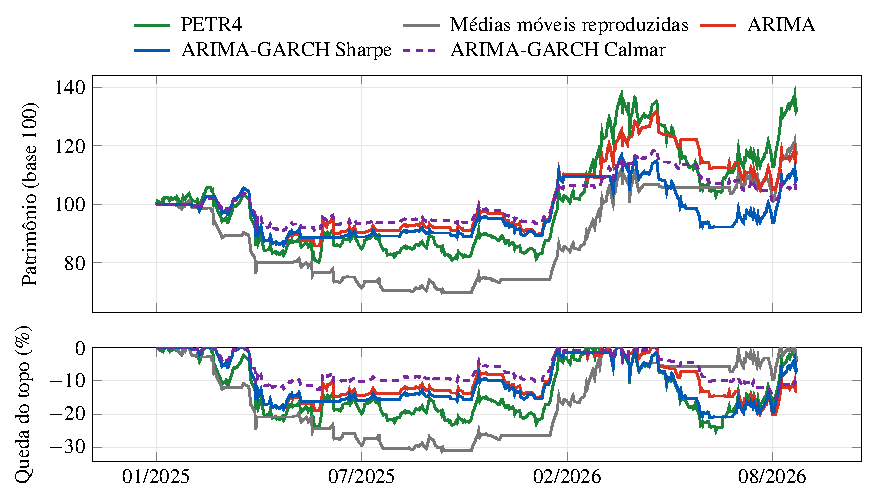
\includegraphics{curva_T3.pdf}
\fonte{Elaboração própria.}
\nota{Resultado bruto, com o capital inicial igual a 100.}
\end{grafico}

O Gráfico~\ref{gra:curva-t3-j} mostra a evolução do patrimônio no período. No saldo
registrado pelo MetaTrader 5, no Gráfico~\ref{gra:mt5-t3-j}, o ARIMA chegou a
R\$ 86 mil em junho de 2025 e a R\$ 128 mil em abril de 2026. O ARIMA-GARCH
Sharpe chegou a R\$ 89 mil em maio de 2025 e terminou com R\$ 109 mil.

\begin{grafico}[htbp]
\centering
\caption{Saldo registrado pelo MetaTrader 5, 2025 a 2026, com janelas fixas}
\label{gra:mt5-t3-j}
{\small ARIMA}\\[2pt]
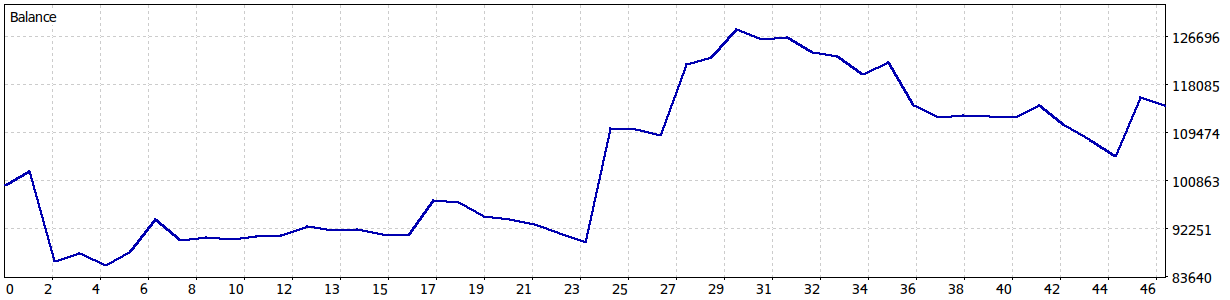
\includegraphics[width=0.7\textwidth]{../relatorios_mt5/rel_R3_T3_AS.png}\\[6pt]
{\small ARIMA-GARCH Sharpe}\\[2pt]
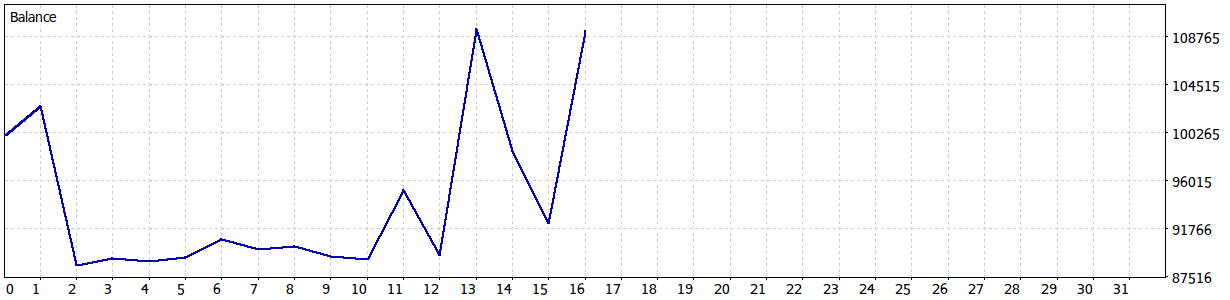
\includegraphics[width=0.7\textwidth]{../relatorios_mt5/rel_R3_T3_GS.png}
\fonte{Relatório do testador de estratégias do MetaTrader 5.}
\nota{Saldo em reais após cada negociação encerrada. O eixo horizontal é o número da negociação, e as escalas dos dois painéis são diferentes.}
\end{grafico}

\section{O efeito vem do GARCH?}
\label{sec:efeito-garch-j}

Cada versão foi comparada com a mesma configuração com o GARCH desligado. Com as
configurações fixas, são doze comparações, reunidas na
Tabela~\ref{tab:efeito-j}. Na versão atual eram onze, porque em 2007 a 2011 os dois
critérios tinham escolhido a mesma configuração.

\begin{table}[htbp]
\centering
\caption{Cada versão com e sem o GARCH, com janelas fixas}
\label{tab:efeito-j}
\fontsize{10}{12}\selectfont
\begin{tabular}{l|l|c|c|c}
\hline
& & Retorno & Queda máx. & Volatilidade \\
Período & ARIMA-GARCH & com / sem & com / sem & com / sem \\
\hline
2007 a 2011 & Sharpe & +31,4\% / $-$12,7\% & 13,5\% / 45,1\% & 12,7\% / 27,5\% \\
\hline
2007 a 2011 & Calmar & +1,7\% / $-$12,7\% & 10,1\% / 45,1\% & 8,4\% / 27,5\% \\
\hline
2013 a 2016 & Sharpe & $-$24,5\% / $-$9,7\% & 77,6\% / 51,9\% & 47,2\% / 35,1\% \\
\hline
2013 a 2016 & Calmar & $-$9,6\% / $-$9,7\% & 40,5\% / 51,9\% & 16,6\% / 35,1\% \\
\hline
2017 a 2024 & Sharpe & +64,6\% / +95,7\% & 37,0\% / 40,5\% & 26,9\% / 32,0\% \\
\hline
2017 a 2024 & Calmar & $-$15,4\% / +4,6\% & 21,6\% / 57,7\% & 4,4\% / 32,6\% \\
\hline
2025 a 2026 & Sharpe & +9,3\% / +14,2\% & 21,1\% / 20,1\% & 22,5\% / 22,0\% \\
\hline
2025 a 2026 & Calmar & +5,3\% / +14,2\% & 15,4\% / 20,1\% & 13,4\% / 22,0\% \\
\hline
2005 a 2026, fixa & Sharpe & +63,0\% / $-$13,6\% & 79,6\% / 83,2\% & 34,5\% / 28,7\% \\
\hline
2005 a 2026, fixa & Calmar & +32,1\% / $-$13,6\% & 44,3\% / 83,2\% & 14,4\% / 28,7\% \\
\hline
2017 a 2024, fixa & Sharpe & +29,3\% / +4,6\% & 62,5\% / 57,7\% & 33,3\% / 32,6\% \\
\hline
2017 a 2024, fixa & Calmar & +7,9\% / +4,6\% & 31,6\% / 57,7\% & 13,6\% / 32,6\% \\
\hline
\end{tabular}
\fonte{Elaboração própria.}
\nota{Resultado bruto. Em cada linha, \textit{com} é a versão escolhida e \textit{sem} é a mesma configuração com o GARCH desligado. As versões fixas começam em fevereiro de 2005.}
\end{table}

A versão com GARCH teve queda máxima menor em nove das doze comparações e
volatilidade menor em oito. No retorno, rendeu mais em sete e menos em cinco. As
comparações em que o GARCH não reduziu a queda máxima ou a volatilidade têm uma
coisa em comum. Todas são
do ARIMA-GARCH Sharpe com só o filtro e com a posição mantida durante o veto, em
2013 a 2016, em 2025 e 2026 e nas duas configurações fixas. Nas oito comparações
em que o GARCH ajusta o tamanho da posição ou encerra a posição no veto, a queda
máxima e a volatilidade foram sempre menores com ele.

O mesmo padrão aparece nas quatro ações quando se olham todas as configurações da
otimização. Entre as que tiram capital do mercado quando a volatilidade sobe, o
GARCH reduziu a queda máxima em 86\% a 95\% das comparações em 2007 a 2011 e em
86\% a 100\% em 2013 a 2016, conforme a ação. Em 2025 e 2026, o efeito foi menor,
de 48\% a 86\%. Entre as que apenas impedem novas compras e mantêm a posição
aberta, a proporção variou de 21\% a 88\%, sem padrão.

Na comparação com as médias móveis, as versões com GARCH oscilaram menos em todos
os períodos, com uma exceção, o ARIMA-GARCH Sharpe de 2013 a 2016. Em 2025 e
2026, porém, a diferença do ARIMA-GARCH Sharpe foi mínima, 22,5\% contra 22,7\%. As médias móveis
renderam mais que as duas versões em 2013 a 2016 e em 2025 e 2026.

\section{Como o GARCH protege}
\label{sec:mecanismo-j}

A taxa de acerto dos robôs com ARIMA, com e sem o GARCH, ficou entre 39,5\% e
56,7\%, e a diferença entre cada versão e a mesma configuração sem o GARCH foi de
no máximo 6,4 pontos percentuais. Como na versão atual, o GARCH não melhorou o
acerto de forma consistente. O $d$ escolhido pelo teste ADF também variou. No
acompanhamento diário do ARIMA-GARCH Sharpe de 2017 a 2024, ele foi 1 em 1.857
dos 1.983 pregões, ou 93,6\%, e 0 nos demais.

O que o GARCH mudou foi a quantidade de capital aplicado. Em 2007 a 2011, o
ARIMA-GARCH Sharpe aplicou em média 21,7\% do patrimônio na ação, contra 43,3\% da
mesma configuração sem o GARCH. Em 2017 a 2024, vetou 428 dos 1.983 sinais do
ARIMA e aplicou 50,7\%, contra 62,3\%. Quando o veto mantém a posição aberta, o
efeito pode se inverter, como em 2013 a 2016, em que o ARIMA-GARCH Sharpe ficou
com 59,4\% aplicado, contra 49,5\% sem o GARCH.

O episódio de 3 de abril de 2020 se repete. Na abertura daquele dia, o ARIMA do
ARIMA-GARCH Sharpe previa alta de 2,16\% e, sozinho, teria comprado. A volatilidade
prevista pelo GARCH era de 7,81\%, cerca de 2,6 vezes o limiar vigente, de 3,01\%,
e a operação foi vetada. No fechamento anterior, a ação acumulava queda de 48,6\%
em relação ao fim de 2019.

% Procedência: C/outras_acoes.txt (VALE3, USIM5 e POMO4); quatro ações: C/analise_grades_cru.txt.
\section{Outras ações}

A Tabela~\ref{tab:outras-j} mostra o resultado bruto das configurações escolhidas
nas outras três ações, com as janelas fixas.

\begin{table}[htbp]
\centering
\caption{Retorno e queda máxima em outras ações, com janelas fixas}
\label{tab:outras-j}
\fontsize{10}{12}\selectfont
\begin{tabular}{l|l|c|c|c|c}
\hline
& & ARIMA & ARIMA-GARCH & ARIMA-GARCH & Ação \\
Ação & Período & & Sharpe & Calmar & \\
\hline
\multirow{3}{*}{VALE3} & 2007 a 2011 & $-$12,5\% / 42,6\% & +1,5\% / 19,2\% & $-$29,1\% / 34,0\% & +23,9\% / 67,7\% \\
 & 2013 a 2016 & +34,2\% / 34,3\% & +7,2\% / 24,9\% & +0,2\% / 8,1\% & $-$40,3\% / 79,9\% \\
 & 2025 a 2026 & +13,4\% / 14,6\% & +20,8\% / 8,3\% & +6,9\% / 17,6\% & +34,1\% / 21,0\% \\
\hline
\multirow{3}{*}{USIM5} & 2007 a 2011 & $-$28,7\% / 67,0\% & $-$43,6\% / 47,0\% & $-$13,1\% / 47,0\% & $-$42,7\% / 79,1\% \\
 & 2013 a 2016 & +0,5\% / 67,6\% & +75,0\% / 44,7\% & sem operações & $-$68,8\% / 94,3\% \\
 & 2025 a 2026 & +22,4\% / 46,3\% & sem operações & sem operações & +29,2\% / 48,1\% \\
\hline
\multirow{3}{*}{POMO4} & 2007 a 2011 & +128,2\% / 39,3\% & $-$0,5\% / 18,7\% & +76,1\% / 12,6\% & +138,3\% / 71,1\% \\
 & 2013 a 2016 & $-$37,9\% / 48,1\% & $-$36,8\% / 47,3\% & $-$15,5\% / 21,6\% & $-$58,0\% / 77,8\% \\
 & 2025 a 2026 & $-$4,9\% / 27,0\% & $-$8,8\% / 10,0\% & $-$1,9\% / 2,4\% & $-$36,2\% / 54,3\% \\
\hline
\end{tabular}
\fonte{Elaboração própria.}
\nota{Resultado bruto. Em cada célula, o retorno e a queda máxima. A ação representa a compra e manutenção, pela variação do preço.}
\end{table}

Em todos os casos em que alguma versão com GARCH operou, a menor queda máxima foi
de uma delas. Só em um caso uma versão com GARCH caiu mais que o ARIMA, o
ARIMA-GARCH Calmar na VALE3 de 2025 e 2026. No retorno não houve padrão, e o maior
ganho da tabela foi de novo do ARIMA, na POMO4 de 2007 a 2011.

A venda a descoberto, simulada em todas as configurações, aumentou a queda máxima
nos doze casos de ação e período e reduziu o retorno em sete deles, considerando a
mediana das comparações de cada caso, o mesmo resultado da versão atual.

% Procedência: E/comparacao_tg.txt (TG = refeito_2026-10-05/testes; estudo =
% E/testes), C/traco_resumo.txt e C/efeito_janela_garch.txt (inclui a conferência
% das 96 passagens sem GARCH).
\section{Comparação com a versão atual}
\label{sec:comparacao-j}

A Tabela~\ref{tab:comparacao-j} reúne o resultado das duas versões com GARCH na
versão atual e com as janelas fixas.

\begin{table}[htbp]
\centering
\caption{Retorno e queda máxima na versão atual e com janelas fixas}
\label{tab:comparacao-j}
\fontsize{10}{12}\selectfont
\begin{tabular}{l|l|c|c}
\hline
Período & ARIMA-GARCH & Versão atual & Janelas fixas \\
\hline
2007 a 2011 & Sharpe & $-$8,4\% / 17,5\% & +31,4\% / 13,5\% \\
\hline
2007 a 2011 & Calmar & $-$8,4\% / 17,5\% & +1,7\% / 10,1\% \\
\hline
2013 a 2016 & Sharpe & $-$13,8\% / 28,6\% & $-$24,5\% / 77,6\% \\
\hline
2013 a 2016 & Calmar & $-$6,8\% / 15,5\% & $-$9,6\% / 40,5\% \\
\hline
2017 a 2024 & Sharpe & +199,5\% / 27,2\% & +64,6\% / 37,0\% \\
\hline
2017 a 2024 & Calmar & +42,9\% / 40,2\% & $-$15,4\% / 21,6\% \\
\hline
2025 a 2026 & Sharpe & $-$13,7\% / 17,6\% & +9,3\% / 21,1\% \\
\hline
2025 a 2026 & Calmar & $-$7,4\% / 12,2\% & +5,3\% / 15,4\% \\
\hline
\end{tabular}
\fonte{Elaboração própria.}
\nota{Resultado bruto. Em cada célula, o retorno e a queda máxima.}
\end{table}

Em sete das oito linhas, a configuração escolhida mudou. A exceção é o
ARIMA-GARCH Sharpe de 2017 a 2024, que nas duas versões é o filtro com percentil
70 que encerra a posição no veto. Ali, a passagem de +199,5\% para +64,6\% vem
só da janela do GARCH. Para separar o efeito da escolha do efeito da janela nos
outros períodos, cada configuração da grade com o ARIMA de 240
pregões foi comparada consigo mesma, com o GARCH sobre os resíduos da janela do
ARIMA, como na versão atual, e sobre 500 resíduos. Nas quatro ações e nos três
períodos, a mediana da diferença na queda máxima ficou entre $-$2,8 e +1,8
pontos percentuais em 22 dos 24 grupos. Somando todos os 3.648 pares, a janela de
500 reduziu a queda máxima em 46,8\% deles, aumentou em 43,8\% e não a mudou nos
demais. As configurações sem GARCH deram exatamente o
mesmo resultado nas duas versões. Nesses períodos, portanto, trocar a janela do GARCH
quase não muda o resultado de uma mesma configuração, e o que mudou foi a
configuração escolhida na otimização, que com a nova grade passou a preferir, em
vários deles, o filtro que mantém a posição durante o veto. Essa comparação não
cobre 2017 a 2024, cuja grade não foi rodada no período de teste, e ali a mesma
configuração mudou bastante com a janela.

Onde a janela fez diferença foi na estimação do próprio GARCH. Entre julho de 2019
e junho de 2021, com os resíduos da janela do ARIMA, a soma $\alpha_1 + \beta_1$
ficou acima de 0,999, encostada no limite que garante a estacionariedade, em
29,0\% dos pregões. Com 500 resíduos, isso aconteceu em 2,2\% dos pregões do mesmo
intervalo e em 1,3\% de todo o período de 2017 a 2024. O $\alpha_1$ mediano caiu de
0,31 para 0,22 no mesmo intervalo e foi de 0,12 no período inteiro. É o
comportamento esperado quando a amostra é pequena para a máxima verossimilhança,
e é o que a janela de 500 reduz.
